\begin{frame}{\small Passive Global Localisation: επιλύσιμο μέσω \texttt{sm2}}

  \begin{figure}
    
\tikzset{every picture/.style={line width=0.75pt}} %set default line width to 0.75pt

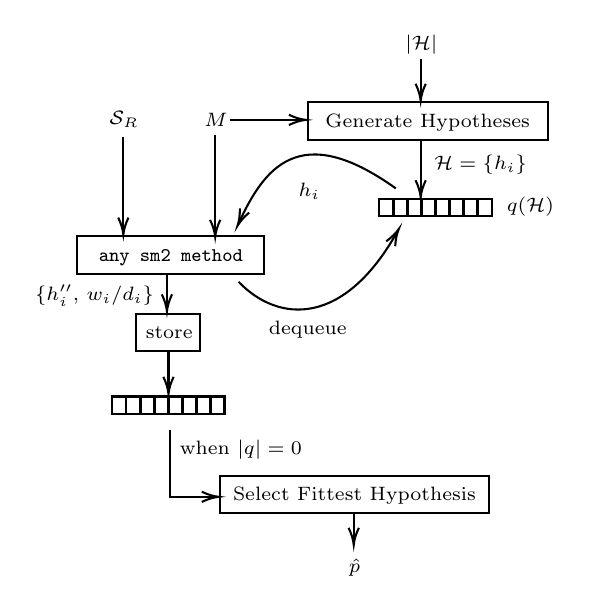
\begin{tikzpicture}[x=0.75pt,y=0.75pt,yscale=-0.75,xscale=0.75]
\scriptsize
%uncomment if require: \path (0,447); %set diagram left start at 0, and has height of 447

%Straight Lines [id:da7180108526379969]
\draw    (108.5,68) -- (108.5,129) ;
\draw [shift={(108.5,131)}, rotate = 270] [color={rgb, 255:red, 0; green, 0; blue, 0 }  ][line width=0.75]    (10.93,-3.29) .. controls (6.95,-1.4) and (3.31,-0.3) .. (0,0) .. controls (3.31,0.3) and (6.95,1.4) .. (10.93,3.29)   ;
%Straight Lines [id:da03009202516620957]
\draw    (299.5,70) -- (299.5,86) -- (299.5,105) ;
\draw [shift={(299.5,107)}, rotate = 270] [color={rgb, 255:red, 0; green, 0; blue, 0 }  ][line width=0.75]    (10.93,-3.29) .. controls (6.95,-1.4) and (3.31,-0.3) .. (0,0) .. controls (3.31,0.3) and (6.95,1.4) .. (10.93,3.29)   ;
%Curve Lines [id:da7710107431830926]
\draw    (182.5,161.29) .. controls (208.37,188.15) and (250.58,190.27) .. (284.98,128.23) ;
\draw [shift={(285.5,127.29)}, rotate = 478.71] [color={rgb, 255:red, 0; green, 0; blue, 0 }  ][line width=0.75]    (10.93,-3.29) .. controls (6.95,-1.4) and (3.31,-0.3) .. (0,0) .. controls (3.31,0.3) and (6.95,1.4) .. (10.93,3.29)   ;
%Straight Lines [id:da8319074018571286]
\draw    (167.5,67) -- (167.5,120) -- (167.5,130.43) ;
\draw [shift={(167.5,132.43)}, rotate = 270] [color={rgb, 255:red, 0; green, 0; blue, 0 }  ][line width=0.75]    (10.93,-3.29) .. controls (6.95,-1.4) and (3.31,-0.3) .. (0,0) .. controls (3.31,0.3) and (6.95,1.4) .. (10.93,3.29)   ;
%Straight Lines [id:da9443063587697282]
\draw    (299.5,18) -- (299.5,34) -- (299.5,43) ;
\draw [shift={(299.5,45)}, rotate = 270] [color={rgb, 255:red, 0; green, 0; blue, 0 }  ][line width=0.75]    (10.93,-3.29) .. controls (6.95,-1.4) and (3.31,-0.3) .. (0,0) .. controls (3.31,0.3) and (6.95,1.4) .. (10.93,3.29)   ;
%Curve Lines [id:da9475685171094514]
\draw    (182.75,123.33) .. controls (198.68,89.07) and (221.06,56.63) .. (283.5,101.29) ;
\draw [shift={(181.79,125.43)}, rotate = 294.57] [color={rgb, 255:red, 0; green, 0; blue, 0 }  ][line width=0.75]    (10.93,-3.29) .. controls (6.95,-1.4) and (3.31,-0.3) .. (0,0) .. controls (3.31,0.3) and (6.95,1.4) .. (10.93,3.29)   ;
%Straight Lines [id:da7873103370093042]
\draw    (176.79,57.29) -- (223.79,57.29) ;
\draw [shift={(225.79,57.29)}, rotate = 180] [color={rgb, 255:red, 0; green, 0; blue, 0 }  ][line width=0.75]    (10.93,-3.29) .. controls (6.95,-1.4) and (3.31,-0.3) .. (0,0) .. controls (3.31,0.3) and (6.95,1.4) .. (10.93,3.29)   ;
%Shape: Rectangle [id:dp9316400431844878]
\draw   (273,108) -- (282.5,108) -- (282.5,119.29) -- (273,119.29) -- cycle ;
%Shape: Rectangle [id:dp2562271025125258]
\draw   (282,108) -- (291.5,108) -- (291.5,119.29) -- (282,119.29) -- cycle ;

%Shape: Rectangle [id:dp39303754153535886]
\draw   (291,108) -- (300.5,108) -- (300.5,119.29) -- (291,119.29) -- cycle ;
%Shape: Rectangle [id:dp6791562149193224]
\draw   (300,108) -- (309.5,108) -- (309.5,119.29) -- (300,119.29) -- cycle ;

%Shape: Rectangle [id:dp5956961748100666]
\draw   (309,108) -- (318.5,108) -- (318.5,119.29) -- (309,119.29) -- cycle ;
%Shape: Rectangle [id:dp03638414398094558]
\draw   (318,108) -- (327.5,108) -- (327.5,119.29) -- (318,119.29) -- cycle ;

%Shape: Rectangle [id:dp7241945812745509]
\draw   (327,108) -- (336.5,108) -- (336.5,119.29) -- (327,119.29) -- cycle ;
%Shape: Rectangle [id:dp30493977014241125]
\draw   (336,108) -- (345.5,108) -- (345.5,119.29) -- (336,119.29) -- cycle ;


%Straight Lines [id:da5492785297164644]
\draw    (256.5,310.29) -- (256.5,328.29) ;
\draw [shift={(256.5,330.29)}, rotate = 270] [color={rgb, 255:red, 0; green, 0; blue, 0 }  ][line width=0.75]    (10.93,-3.29) .. controls (6.95,-1.4) and (3.31,-0.3) .. (0,0) .. controls (3.31,0.3) and (6.95,1.4) .. (10.93,3.29)   ;
%Straight Lines [id:da8400249545776366]
\draw    (138.5,256.43) -- (138.5,299.43) -- (167.79,299.43) ;
\draw [shift={(169.79,299.43)}, rotate = 180] [color={rgb, 255:red, 0; green, 0; blue, 0 }  ][line width=0.75]    (10.93,-3.29) .. controls (6.95,-1.4) and (3.31,-0.3) .. (0,0) .. controls (3.31,0.3) and (6.95,1.4) .. (10.93,3.29)   ;
%Shape: Rectangle [id:dp36899940738692605]
\draw   (101,235) -- (110.5,235) -- (110.5,246.29) -- (101,246.29) -- cycle ;
%Shape: Rectangle [id:dp3740402995546943]
\draw   (110,235) -- (119.5,235) -- (119.5,246.29) -- (110,246.29) -- cycle ;

%Shape: Rectangle [id:dp9204771715668112]
\draw   (119,235) -- (128.5,235) -- (128.5,246.29) -- (119,246.29) -- cycle ;
%Shape: Rectangle [id:dp2611557502938522]
\draw   (128,235) -- (137.5,235) -- (137.5,246.29) -- (128,246.29) -- cycle ;

%Shape: Rectangle [id:dp5918549750705964]
\draw   (137,235) -- (146.5,235) -- (146.5,246.29) -- (137,246.29) -- cycle ;
%Shape: Rectangle [id:dp7742676605094942]
\draw   (146,235) -- (155.5,235) -- (155.5,246.29) -- (146,246.29) -- cycle ;

%Shape: Rectangle [id:dp4802635551676304]
\draw   (155,235) -- (164.5,235) -- (164.5,246.29) -- (155,246.29) -- cycle ;
%Shape: Rectangle [id:dp005738431700191393]
\draw   (164,235) -- (173.5,235) -- (173.5,246.29) -- (164,246.29) -- cycle ;


%Straight Lines [id:da2941675174511593]
\draw    (136.5,156.29) -- (136.5,178.29) ;
\draw [shift={(136.5,180.29)}, rotate = 270] [color={rgb, 255:red, 0; green, 0; blue, 0 }  ][line width=0.75]    (10.93,-3.29) .. controls (6.95,-1.4) and (3.31,-0.3) .. (0,0) .. controls (3.31,0.3) and (6.95,1.4) .. (10.93,3.29)   ;
%Straight Lines [id:da828241073247397]
\draw    (137.5,206.29) -- (137.5,231.29) ;
\draw [shift={(137.5,233.29)}, rotate = 270] [color={rgb, 255:red, 0; green, 0; blue, 0 }  ][line width=0.75]    (10.93,-3.29) .. controls (6.95,-1.4) and (3.31,-0.3) .. (0,0) .. controls (3.31,0.3) and (6.95,1.4) .. (10.93,3.29)   ;

% Text Node
\draw (109,57) node   [align=left] {$\mathcal{S}_R$};
% Text Node
\draw    (227,46) -- (381,46) -- (381,70) -- (227,70) -- cycle  ;
\draw (304,59) node   [align=left] {Generate Hypotheses};
% Text Node
\draw    (79,132) -- (199,132) -- (199,156) -- (79,156) -- cycle  ;
\draw (139,146) node   [align=left] {\texttt{any\ sm2\ method}};
% Text Node
\draw (90,170) node   [align=left] {$\{\bm{h}_i^{\prime\prime}$, $w_i$/$d_i\}$};
% Text Node
\draw (338,86) node   [align=left] {$\mathcal{H} = \{\bm{h}_i\}$};
% Text Node
\draw (168,57) node   [align=left] {$\bm{M}$};
% Text Node
\draw (228,103) node   [align=left] {$\bm{h}_i$};
% Text Node
\draw (227,192) node   [align=left] {dequeue};
% Text Node
\draw (300,9) node   [align=left] {$|\mathcal{H}|$};
% Text Node
\draw    (170.5,286) -- (343.5,286) -- (343.5,310) -- (170.5,310) -- cycle  ;
\draw (257,299) node   [align=left] {Select Fittest Hypothesis};
% Text Node
\draw (370,113) node   [align=left] {$\bm{q}(\mathcal{H})$};
% Text Node
\draw (184,269) node   [align=left] {when $|\bm{q}|=0$};
% Text Node
\draw (257,345) node   [align=left] {$\hat{\bm{p}}$};
% Text Node
\draw    (116.5,182) -- (157.5,182) -- (157.5,206) -- (116.5,206) -- cycle  ;
\draw (138,194) node   [align=left] {store};
\end{tikzpicture}

  \end{figure}

\note{\footnotesize
Το πρόβλημα του passive global localisation μπορεί να λυθεί μέσω οποιασδήποτε τεχνικής
  sm2 ως εξής: δεδομένου του χάρτη $M$ του περιβάλλοντος στο οποίο βρίσκεται το
  φυσικό ρομπότ, διασπείρονται με τυχαίο τρόπο σε αυτόν ένας αριθμός από
  υποθέσεις στάσης $H$, οι οποίες τοποθετούνται σε μία ουρά $q$. Από κάθε υπόθεση
  υπολογίζεται η εικονική σάρωση, και στη συνέχεια μέσω sm2 επιχειρείται η
  ευθυγράμμιση της με τη σάρωση που συλλαμβάνεται από το φυσικό αισθητήρα
  $S_R$. Στο τέλος κάθε ευθυγράμμισης αποθηκεύονται μία υποψήφια τελική
  εκτίμηση στάσης και η τιμή μίας μετρικής που αποτυπώνει το βαθμό ομοιότητας ή
  τελικής ευθυγράμμισης ανάμεσα στην πραγματική σάρωση και την εικονική σάρωση
  που συλλαμβάνεται από κάθε υποψήφια στάση.
  %Για τις τεχνικές sm2 που λειτουργούν με αντιστοιχίσεις αυτό το μέτρο
  %υπολογίζεται εσωτερικά σε κάθε μέθοδο ως το άθροισμα των αποστάσεων των
  %σημειών της μίας σάρωσης ως προς τα σημεία, τις γραμμές ή τις κατανομές της
  %δεύτερης, και στο δικό μας σύστημα αυτό το μέτρο προέρχεται απευθείας από τον
  %FMI-SPOMF.
  Στο τέλος το σύστημα εξάγει ως τελική εκτίμηση στάσης εκείνη που
  σημειώνει τη μεγαλύτερη τιμή ομοιότητας.}

\end{frame}
